\subsection{État de l'art}

Pour les instruments auto-oscillants, on distingue 2 types de modèles physiques permettant la synthèse audio: l'approche modale et l'approche par guide d'ondes.

Les deux approches consistent à, modéliser d'une part le comportement d'un excitateur non linéaire auquel le musicien apporte de l'énergie et d'autre part un résonateur passif linéaire.

$$p = F(q)$$ % cf Mc Intyre et al. mais en vrai je sais pas trop comment finir cette intro là

Dans le cas

% J'ai discuté avec Charlotte et du coup on utilise la même fonction non linéaire entre l'article de Taillard et leur approche modale (modélisation de la dynamique de l'anche)

\subsubsection{Approche modale}

\subsubsection{Approche guide d'ondes}

Le modèle initial de guide d'ondes principalement utilisé par la littérature est celui McIntyre et al. \cite{mcintyre_oscillations_1983}. Dans le cas de la clarinette, la pression et le débit à l'intérieur du résonateur sont séparés en ondes aller et retour. 
A l'aide d'une fonction de réflexion qui peut être déduite de l'impédance d'entrée du résonateur, on peut exprimer l'onde retour en fonction de l'onde aller : $p^-(t) = [r * p^+] (t)$.

Fonction de réflexion :

- dirac

- modèle de Raman \cite{raman1918mechanical}

- tenir compte de la sélectivité en fréquences des pertes et de la dispersion : modèle

% A l'extrémité ouverte de l'instrument, l'onde retour 

Ce modèle est également valable avec les instruments à cordes frottées \cite{ollivier_idealized_2004} en effectuant plusieurs analogies entre les grandeurs physiques propres aux instruments à vents (débit et pression), à celles propres aux instruments à cordes frottées (force au point de jeu et vitesse de la corde).

\paragraph{Fonction non linéaire}

\begin{itemize}
    \item Parabole \cite{mcintyre_oscillations_1983}
    \item $x^3 - x$ \cite{maganza_bifurcations_1986} utilisé pour 
    \item 
\end{itemize}


\subsection{Méthodes et résultats}

On s'intéresse à comparer ces deux approches de modélisation de ces instrument, en terme d'intérêt pour la synthèse sonore, capacité prédictive, différents régimes obtenus.. et explorer l'espace de contrôle. 

\subsubsection{Approche modale}


\begin{figure*}
    \centering
    \begin{subfigure}[b]{.24\linewidth}
        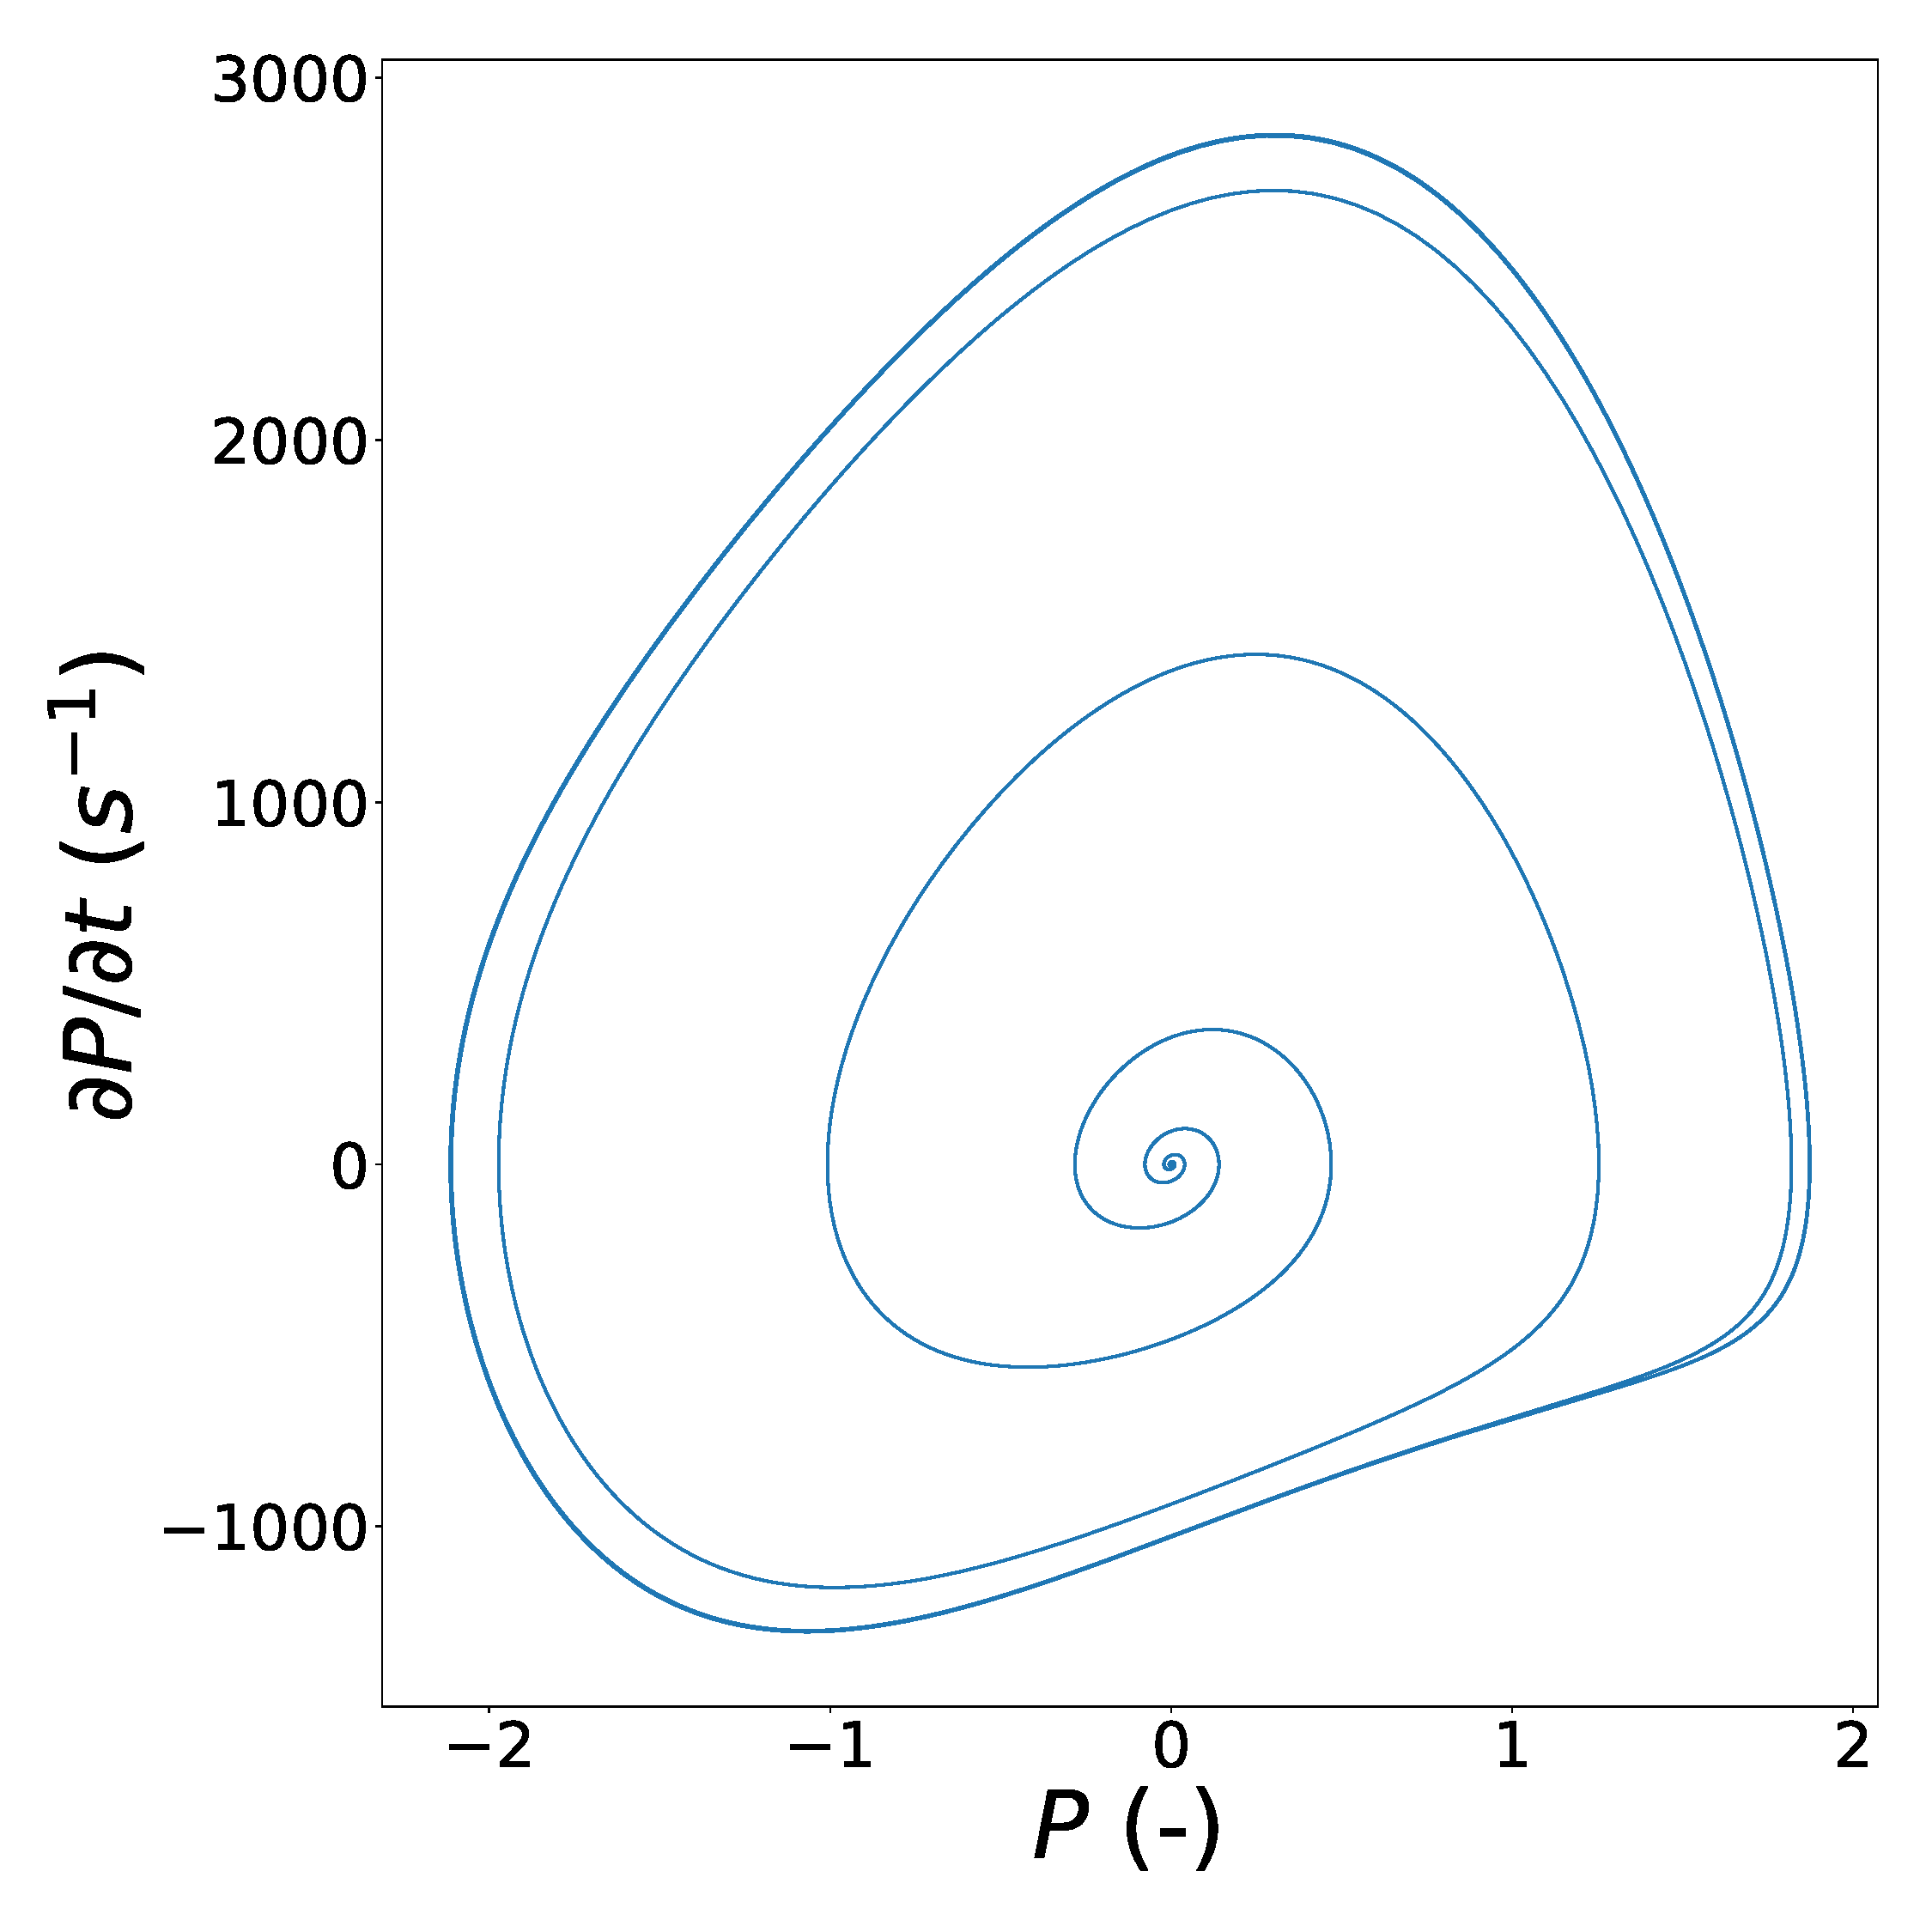
\includegraphics[width=\linewidth]{img/phase_diagram_N1.pdf}
        \caption{$N=1$}
        \label{fig:VDP_phase_N1}
    \end{subfigure}
    \hfill
    \begin{subfigure}[b]{.24\linewidth}
        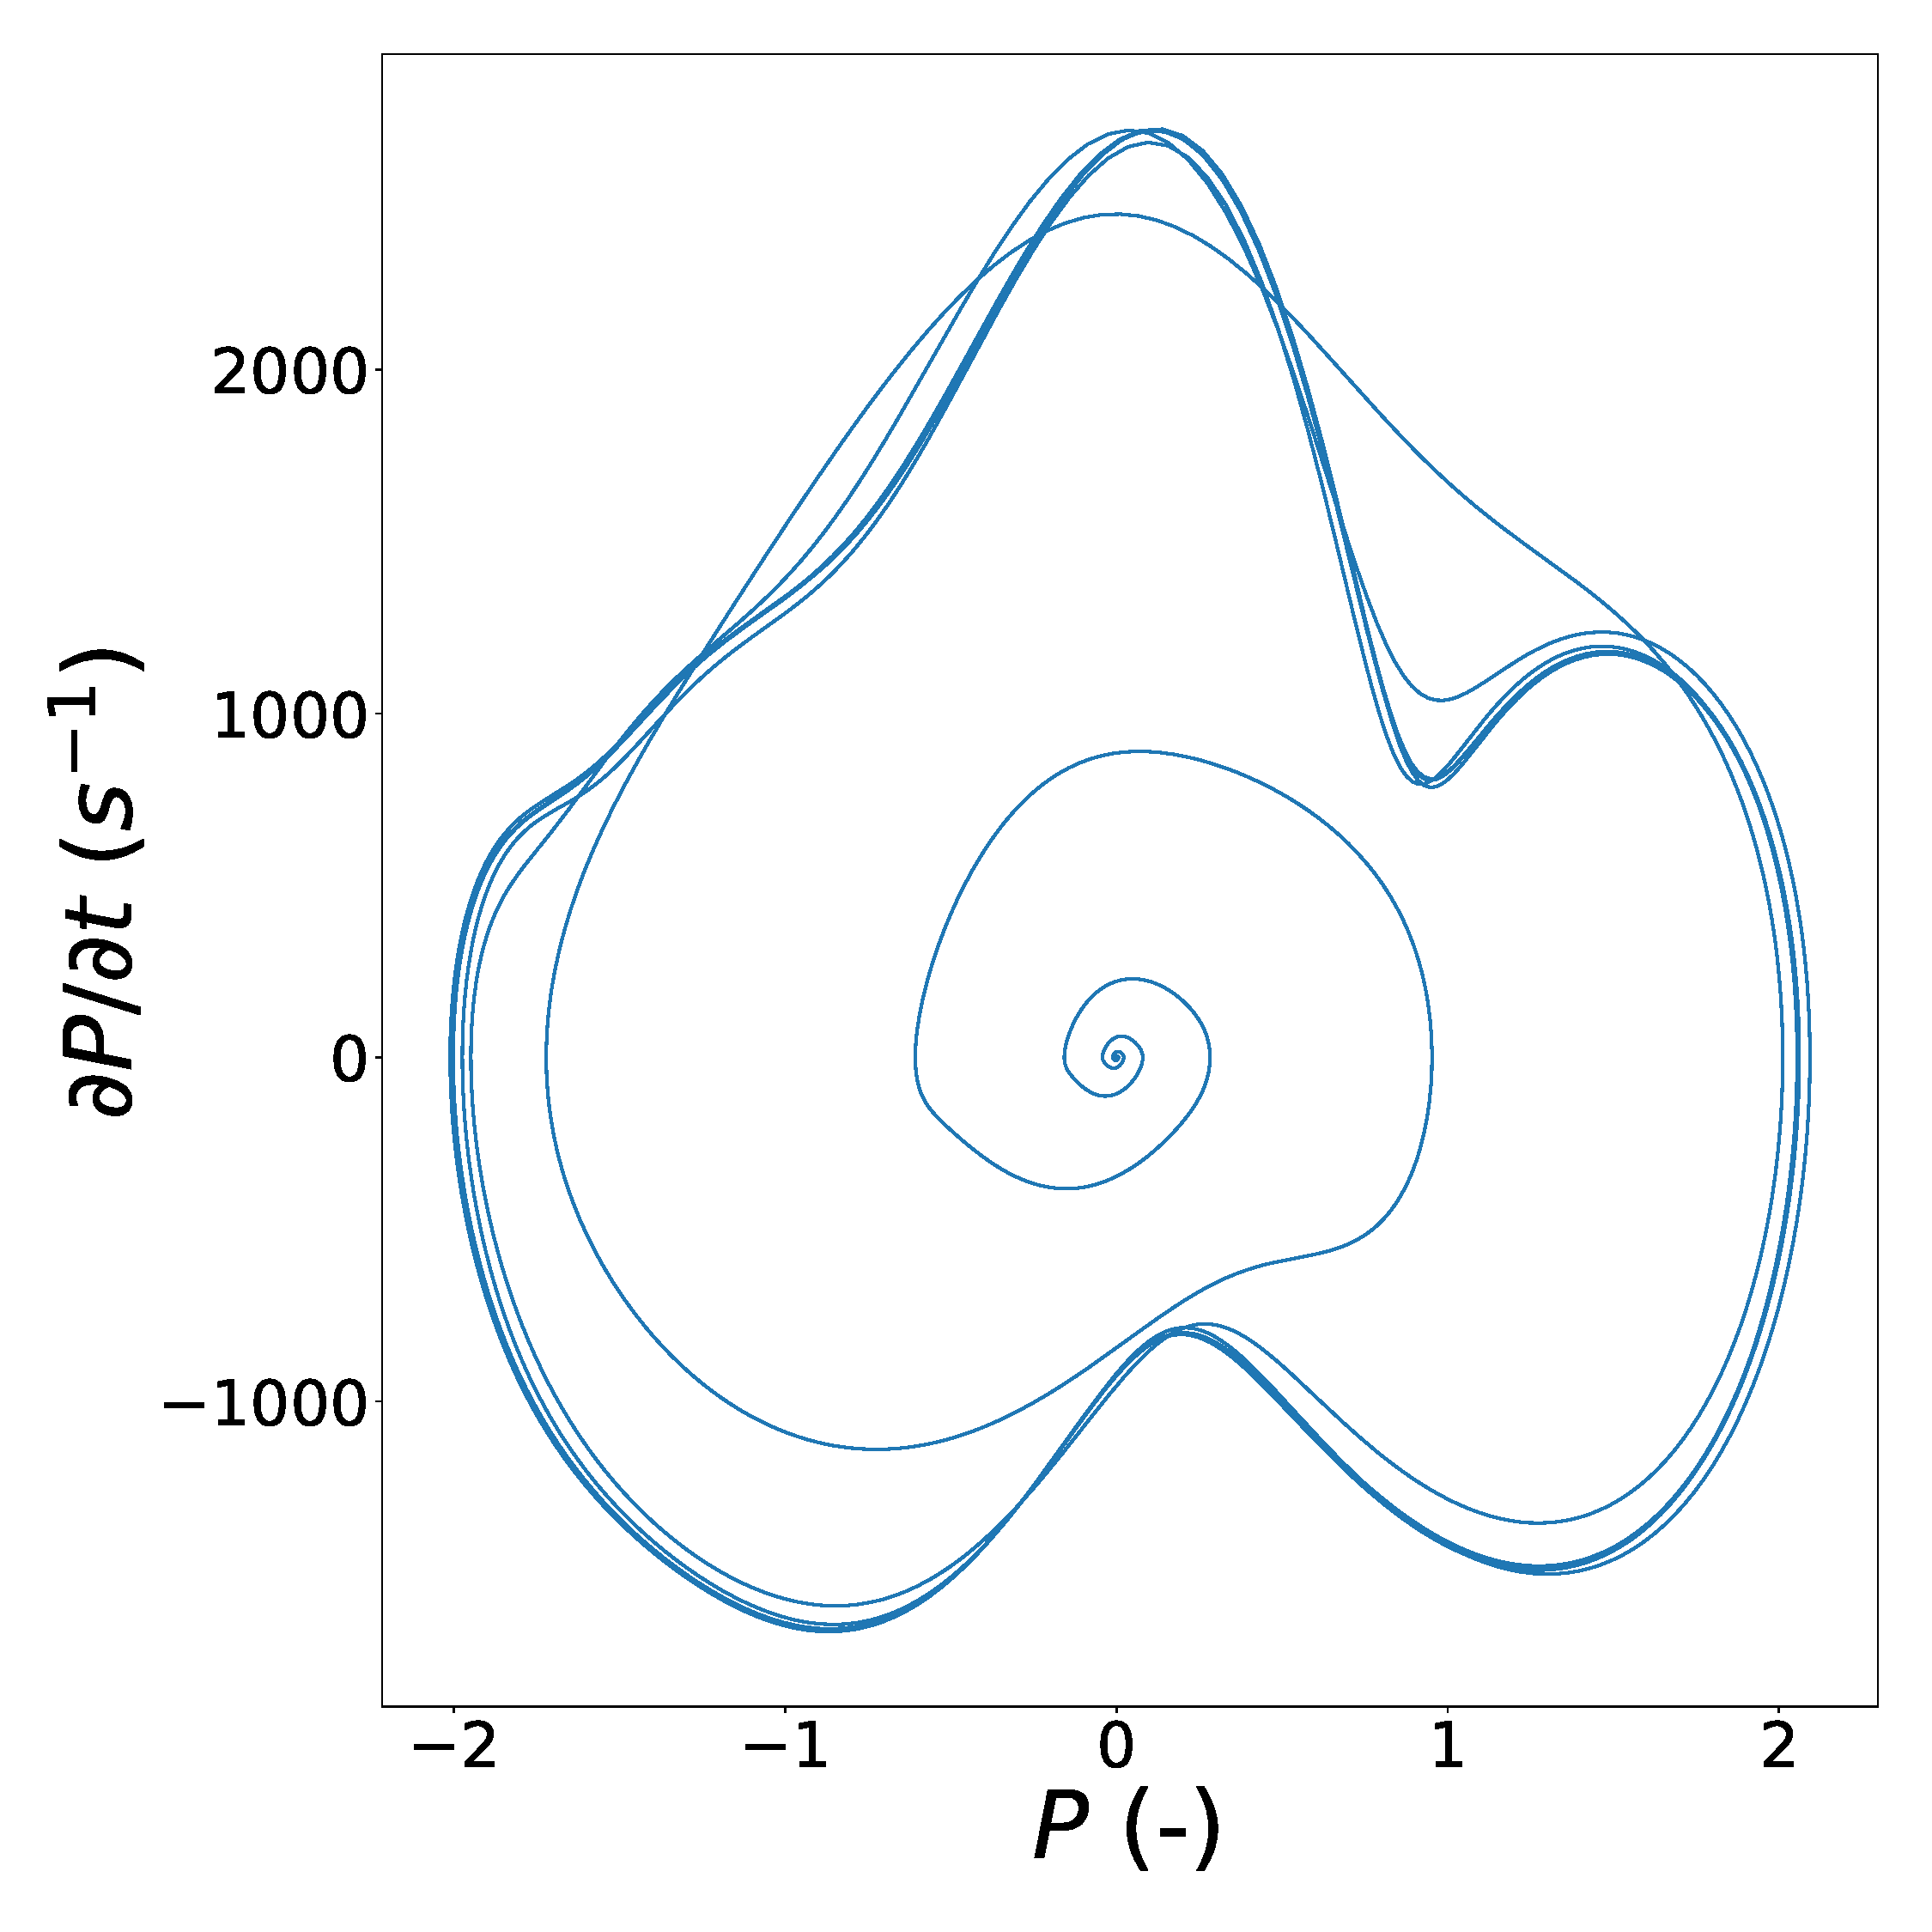
\includegraphics[width=\linewidth]{img/phase_diagram_N2.pdf}
        \caption{$N=2$}
        \label{fig:VDP_phase_N2}
    \end{subfigure}
    \hfill
    \begin{subfigure}[b]{.24\linewidth}
        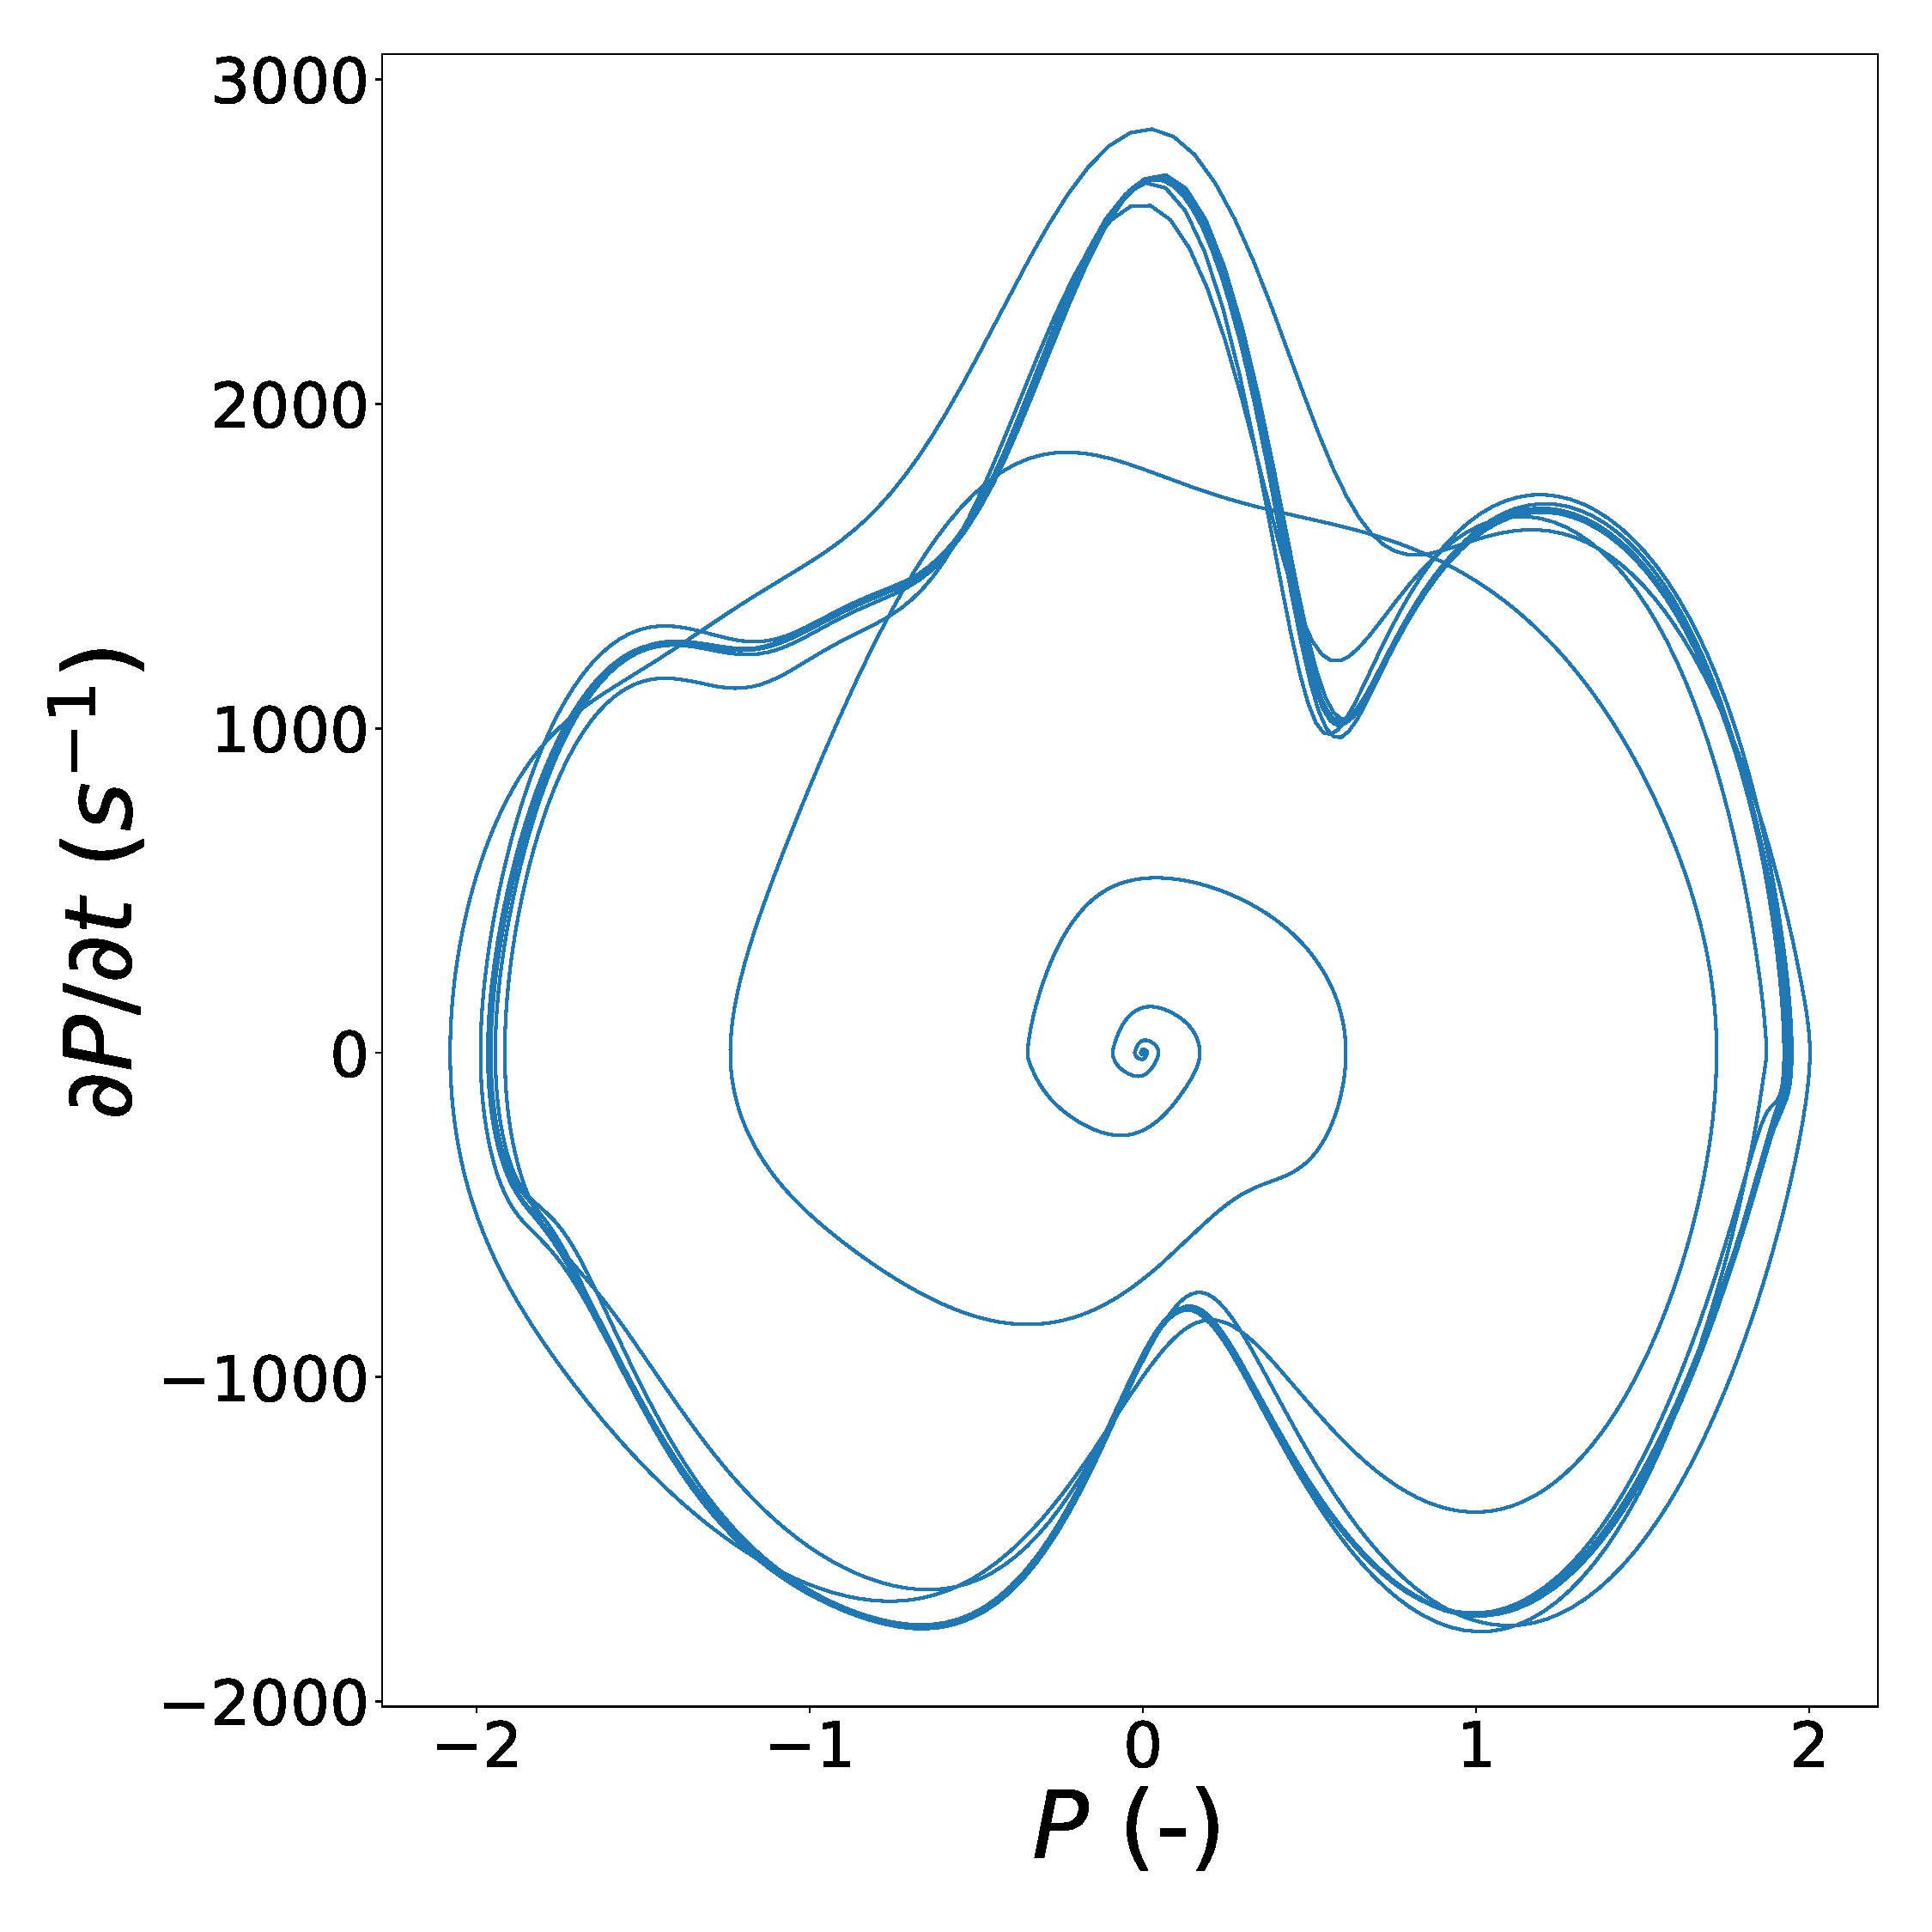
\includegraphics[width=\linewidth]{img/phase_diagram_N3.pdf}
        \caption{$N=3$}
        \label{fig:VDP_phase_N3}
    \end{subfigure}
    \hfill
    \begin{subfigure}[b]{.24\linewidth}
        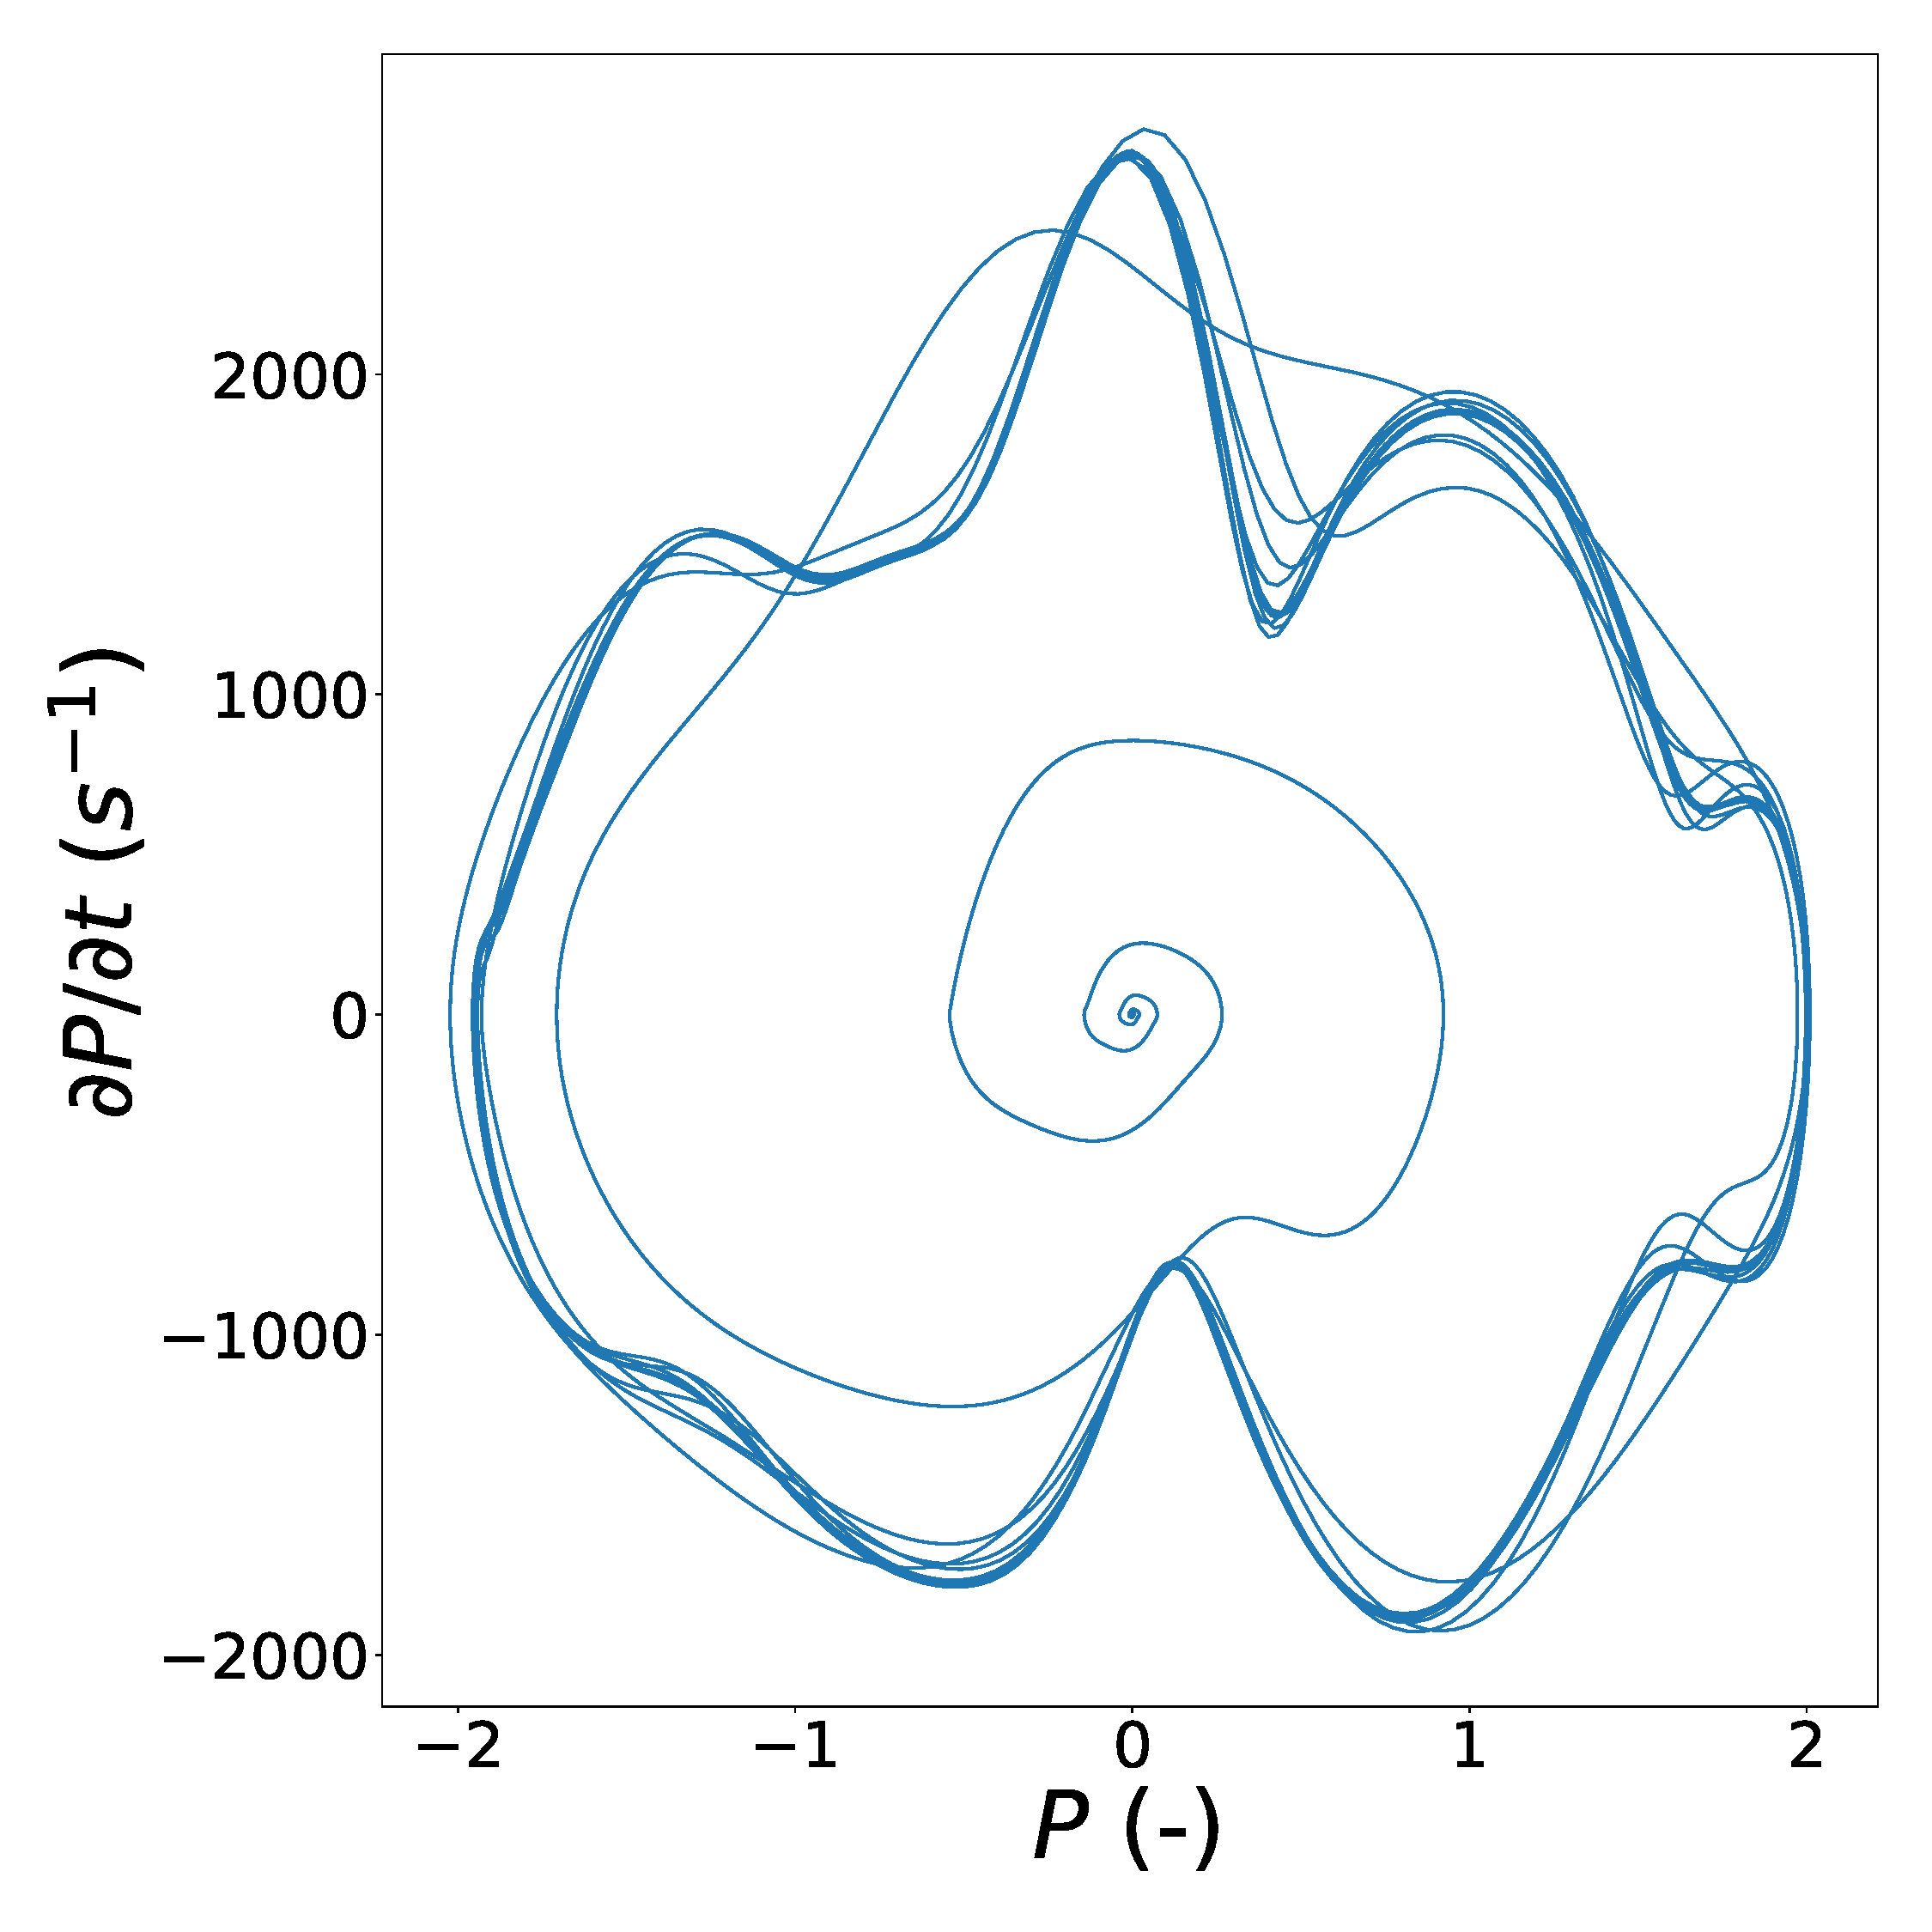
\includegraphics[width=\linewidth]{img/phase_diagram_N4.pdf}
        \caption{$N=4$}
        \label{fig:VDP_phase_N4}
    \end{subfigure}
    \caption{Evolution du flot $(P_0,\frac{\partial P_0}{\partial t})$ dans l'espace des phases durant l'attaque ($t<0.3$ s) pour $N$ modes. Le système est initialement perturbé par un saut de pression $P(t=0)=\epsilon$ ($\epsilon \ll 1$). Les solutions du système d'équations de Van der Pol convergent vers un cycle limite, dont la forme se complexifie avec N.}
    \label{fig:VDP_phase}
\end{figure*}

- résolution numérique : runge kuta

\subsubsection{Cartes itérées}

\subsubsection{Guide d'onde}

Ligne à retard, complexification du modèle pour tenir compte des pertes plus importantes en hautes fréquences.